%%%%%%%%%%%%%%%%%%%%%%%%%%%%%%%%%%%%%%%%%%%%%%%%%%%%%%%%%%%%%%%%%%
%%%%%%%% ICML 2017 EXAMPLE LATEX SUBMISSION FILE %%%%%%%%%%%%%%%%%
%%%%%%%%%%%%%%%%%%%%%%%%%%%%%%%%%%%%%%%%%%%%%%%%%%%%%%%%%%%%%%%%%%

% Use the following line _only_ if you're still using LaTeX 2.09.
%\documentstyle[icml2017,epsf,natbib]{article}
% If you rely on Latex2e packages, like most moden people use this:
\documentclass{article}

% use Times
\usepackage{times}
% For figures
\usepackage{graphicx} % more modern
%\usepackage{epsfig} % less modern
\usepackage{subfigure} 
\usepackage{float}

% For citations
\usepackage{natbib}

% For algorithms
\usepackage{algorithm}
\usepackage{algorithmic}

% For math equations
\usepackage{amsmath}

% As of 2011, we use the hyperref package to produce hyperlinks in the
% resulting PDF.  If this breaks your system, please commend out the
% following usepackage line and replace \usepackage{icml2017} with
% \usepackage[nohyperref]{icml2017} above.
\usepackage{hyperref}

% Packages hyperref and algorithmic misbehave sometimes.  We can fix
% this with the following command.
\newcommand{\theHalgorithm}{\arabic{algorithm}}

% Employ the following version of the ``usepackage'' statement for
% submitting the draft version of the paper for review.  This will set
% the note in the first column to ``Under review.  Do not distribute.''
\usepackage[accepted]{icml2017}

% Employ this version of the ``usepackage'' statement after the paper has
% been accepted, when creating the final version.  This will set the
% note in the first column to ``Proceedings of the...''
%\usepackage[accepted]{icml2017}


% The \icmltitle you define below is probably too long as a header.
% Therefore, a short form for the running title is supplied here:
\icmltitlerunning{Submission and Formatting Instructions for ICML 2017}

\begin{document} 

\twocolumn[
\icmltitle{Variational Neural Conversational Model}

% It is OKAY to include author information, even for blind
% submissions: the style file will automatically remove it for you
% unless you've provided the [accepted] option to the icml2017
% package.

% list of affiliations. the first argument should be a (short)
% identifier you will use later to specify author affiliations
% Academic affiliations should list Department, University, City, Region, Country
% Industry affiliations should list Company, City, Region, Country

% you can specify symbols, otherwise they are numbered in order
% ideally, you should not use this facility. affiliations will be numbered
% in order of appearance and this is the preferred way.
\icmlsetsymbol{equal}{*}

\begin{icmlauthorlist}
\icmlauthor{Xupeng Tong}{equal,to}
\icmlauthor{Chao-Ming Yen}{equal,to}
\icmlauthor{Yikang Li}{equal,to}
\end{icmlauthorlist}

\icmlaffiliation{to}{Carnegie Mellon University, USA}

\icmlcorrespondingauthor{Xupeng Tong}{xtong@andrew.cmu.edu}

% You may provide any keywords that you 
% find helpful for describing your paper; these are used to populate 
% the "keywords" metadata in the PDF but will not be shown in the document
\icmlkeywords{boring formatting information, machine learning, ICML}

\vskip 0.3in
]

% this must go after the closing bracket ] following \twocolumn[ ...

% This command actually creates the footnote in the first column
% listing the affiliations and the copyright notice.
% The command takes one argument, which is text to display at the start of the footnote.
% The \icmlEqualContribution command is standard text for equal contribution.
% Remove it (just {}) if you do not need this facility.

%\printAffiliationsAndNotice{}  % leave blank if no need to mention equal contribution
\printAffiliationsAndNotice{\icmlEqualContribution} % otherwise use the standard text.
%\footnotetext{hi}

\section{Introduction}
Conversation modeling is a famous task that allows the machine to generate reasonable responses according to the sentence it is shown. Previously, a fair amount of works havs been done.

In this project, we plan to improve the model performance based on previous works by incorporating latent information in the model by discovering several existing in variational methods. Especially, we are interested in RNN based variational autoencoder (VAE), that can seamlessly concatenate the seq2seq model with fine-tuned regularization.

By the time we write this midway report, we have produced some preliminary result of our vanilla seq2seq model. We've also implemented the variational auto-encoder, which we have yet not able to integrate the result into our proposed model.

\section{Related Works}
\subsection{Neural Conversational Model}

Sequence To Sequence model is first introduced in \cite{seq2seq}, and since then, has become the standard model for dialogue systems \cite{ncm} and machine translation. It consists of two RNNs (Recurrent Neural Network): An Encoder and a Decoder. The encoder takes a words sequence as input and processes one word at each time step. 

The objective is to convert symbol sequence into a fixed size feature vector that encodes the important information in the sequence while losing the redundant or unnecessary information.

\subsection{Auto-Encoding Variational Bayes}

Variational autoencoder (VAE) \cite{vae} has successfully injected the probabilistic flavor in the basic autoencoder by reparameterization and reconstruction of the outputs as probabilistic random variables within a model and approximate objective function that can conduct end to end training.

Given an observed variable $x$, VAE introduces a continuous latent variable z, and assumes that $x$ is generated from $z$

$$p(x,z) = p(x|z)p(z)$$

The prior over the latent random variables, $p(z)$, is always chosen to be a simple Gaussian distribution and the conditional $p(x|z)$ is an arbitrary observation model whose parameters are computed by a parametric function of $z$. 

In VAE, $p(x|z)$ plays a role as parameterized function approximator (neural network). The generative model $p(x|z)$ and inference model $q(z|x)$ are trained jointly by maximizing the variational lower bound with respect to their parameters, where the integral with respect to $q(z|x)$ is approximated stochastically. The gradient of this estimate can have a low variance estimate, by reparameterizing $z = \mu+\sigma\odot\epsilon$

We can formulate the above problem as minimizing the KL divergence of these two distributions, however, it is generally hard to actually compute it. Alternatively, VAE chooses to optimize some thing that is equivalent to the KL up to an added constant,

$$\text{ELBO}_i (\lambda) = E_{q\lambda (z|x_i)}[\log p(x_i|z)]-KL(q\lambda (z|x_i)||p(z))$$ 

called Evidence Lower BOund (ELBO).

With the perspective from bayesian statistics, the encoder becomes a variational inference network, mapping observed inputs to its approximate posterior distributions over the latent space, while the decoder works as a generative network that maps arbitrary latent coordinates back to distributions over the original space.


\subsection{Variational Recurrent Neural Network}
Earlier works in \cite{vrnn} introduced high-level random latent variables to recurrent neural network (RNN), empowering the model to be able to capture even higher variabilities sequential dataset such as natural speech. Differed from variational auto-encoders (VAE) used for the cases of a non-sequential dataset, where latent random variables were designed to capture the variations in the observed variables. In VRNN, the recurrent network has a VAE for each time step, and these VAEs are conditioned on hidden state variable, such that

$$\bf x_t \bf | z_t \sim \mathcal{N}(\bf \mu _{x,t}, diag(\sigma _{x,t}^2)$$
where,
$$[\bf \mu _{x,t}, \sigma _{x,t}^2] = \varphi^{dec}_{\tau}(\varphi^{\bf z}_{\tau}(\bf z_t),\bf h_{t-1})$$

extract sequential features, and hidden states of RNN can be updated using recurrence equation

\begin{align*}
\bf h_t = f_\theta(\varphi^{\bf x}_\tau (\bf x _t), \varphi^{\bf z}_\tau (\bf z_t), \bf h_{t-1})
\end{align*}

\section{Methods}
\subsection{Seq2Seq model for machine conversation}
To construct a Seq2Seq model for machine conversation, we take similar setting as Google chatbot \cite{ncm}. The model is based on two LSTM layers: one for encoding and the other for decoding, as shown in the original paper of Seq2Sq2 model \cite{seq2seqO}. 

\begin{figure}[H]
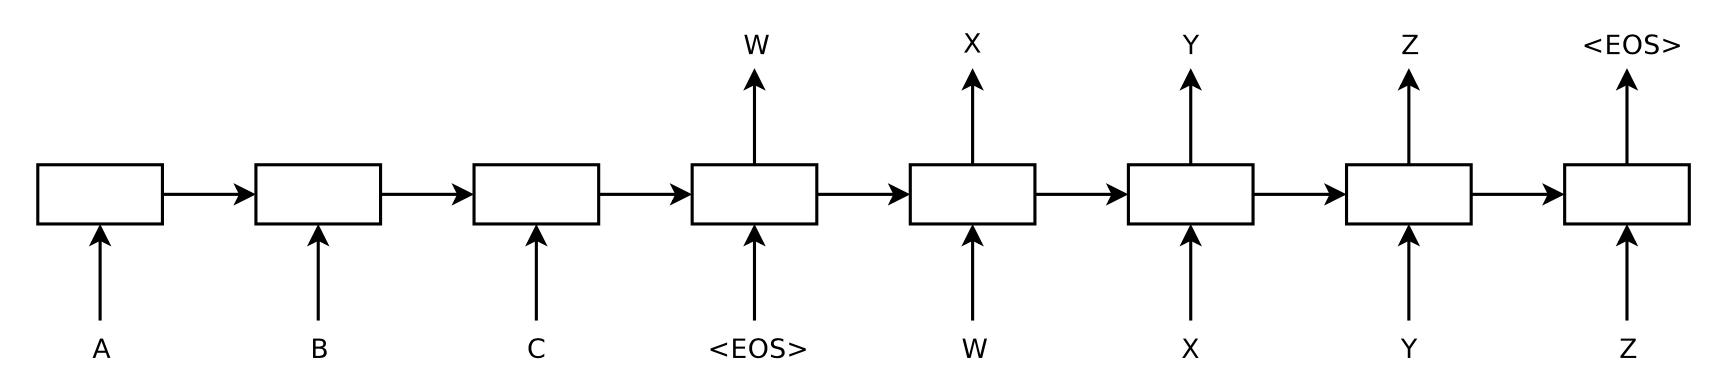
\includegraphics[width=0.4\textwidth]{seq2seq.png}
\caption{Illustration of Seq2Seq model. Figure is taken from the original paper \cite{seq2seqO}.}
\label{fig:seq2seq}
\end{figure}

The sentence is processed token by token, and the input sentence is read in reverse in LSTM, for introducing short-term dependencies in the data to make it easier for optimization \cite{seq2seqO}. The encoding part of the model (A, B, C in the figure) is for input sequence to encode the "thought" of input into a feature vector. The decoding part (W, X, Y, Z) is for generating a response from feature vector. Together we train the model end-to-end with gradient descent optimizer.

\subsection{Incorporating latent information unsupervised as the input to Seq2Seq model}
Applying the vanilla neural conversation model with seq2seq structure has various drawbacks, one of which appears as the respond might not be able to reflect the context, and inconsistency might occur across the conversation.

To solve the above-mentioned problem, we want to train a model that can encode the sentence not only precedes to our expected output, but also the context that the conversation occurs. We consider using Variational Recurrent Auto-Encoder \cite{vrae} that has been successfully applied in encoding the posterior distribution of time series data in \ref{fig:vrae}. The VRAE model shares the same re-parametrization with \cite{vae} while replaces the input and output to LSTM/RNN layers that can better capture the time dependencies.

\begin{figure*}[]
\centering
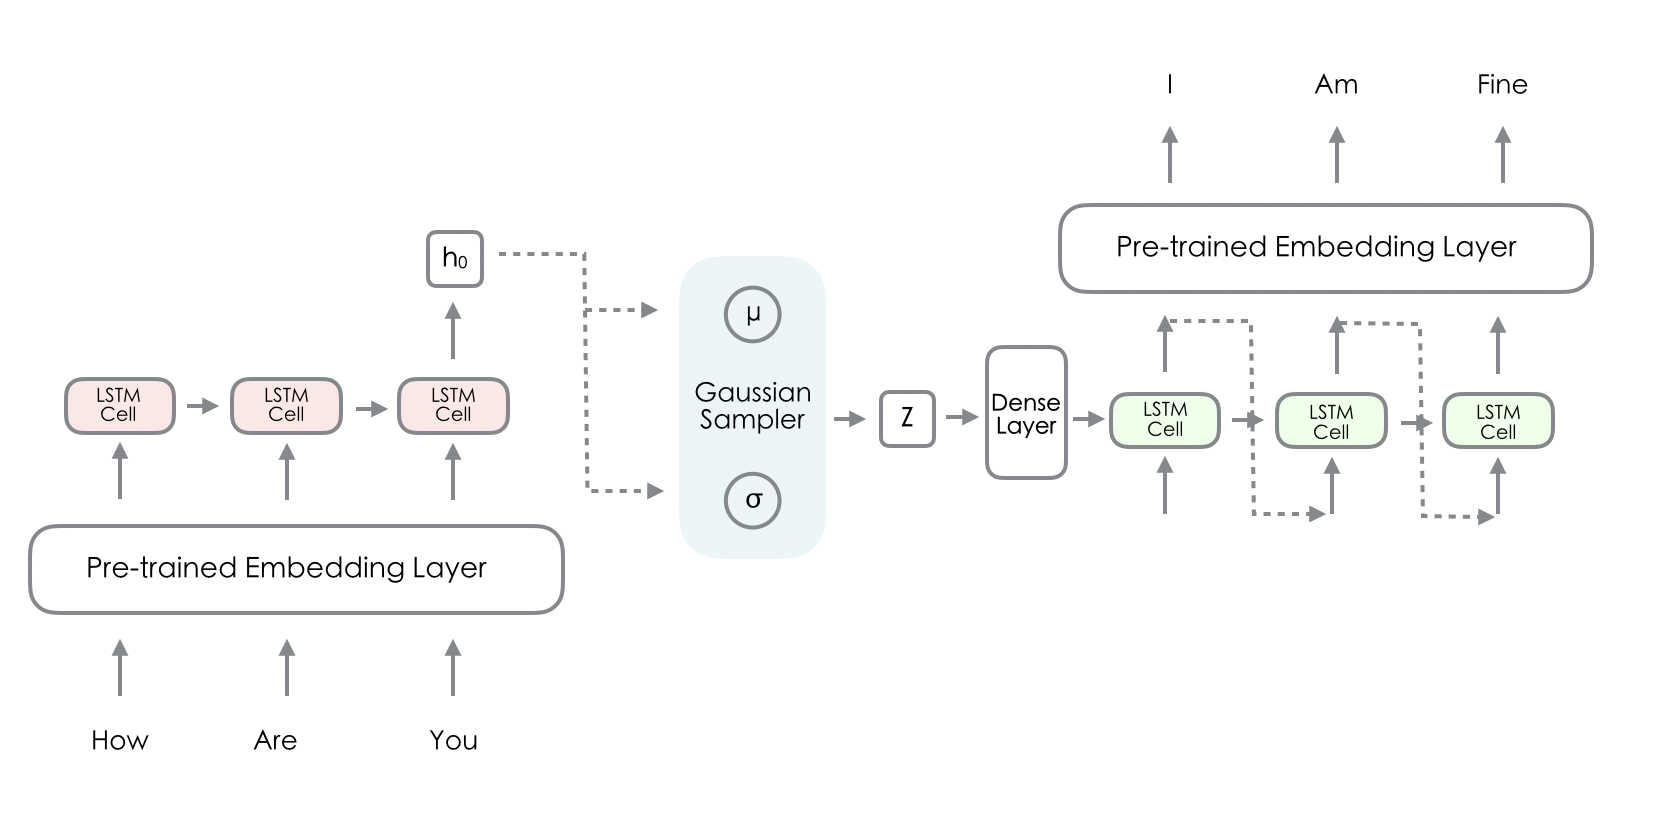
\includegraphics[width=0.8\textwidth]{VRAE.png}
\caption{Variational Recurrent Auto-encoder}
\label{fig:vrae}
\end{figure*}

VRAE can be trained as an independent model with sentences from the same resources of the seq2seq model for sentence prediction. It can be well regarded as another seq2seq model that automatically encodes the side information (context) that assists the core model to perform better predictions. While in the training process for neural conversation model, we use the pre-trained weight of the VRAE as a latent variable extractor, and with context information fed in, it produces the encoded information with which we can concatenate them in our core model, \ref{fig:proposed}.

\begin{figure*}[]
\centering
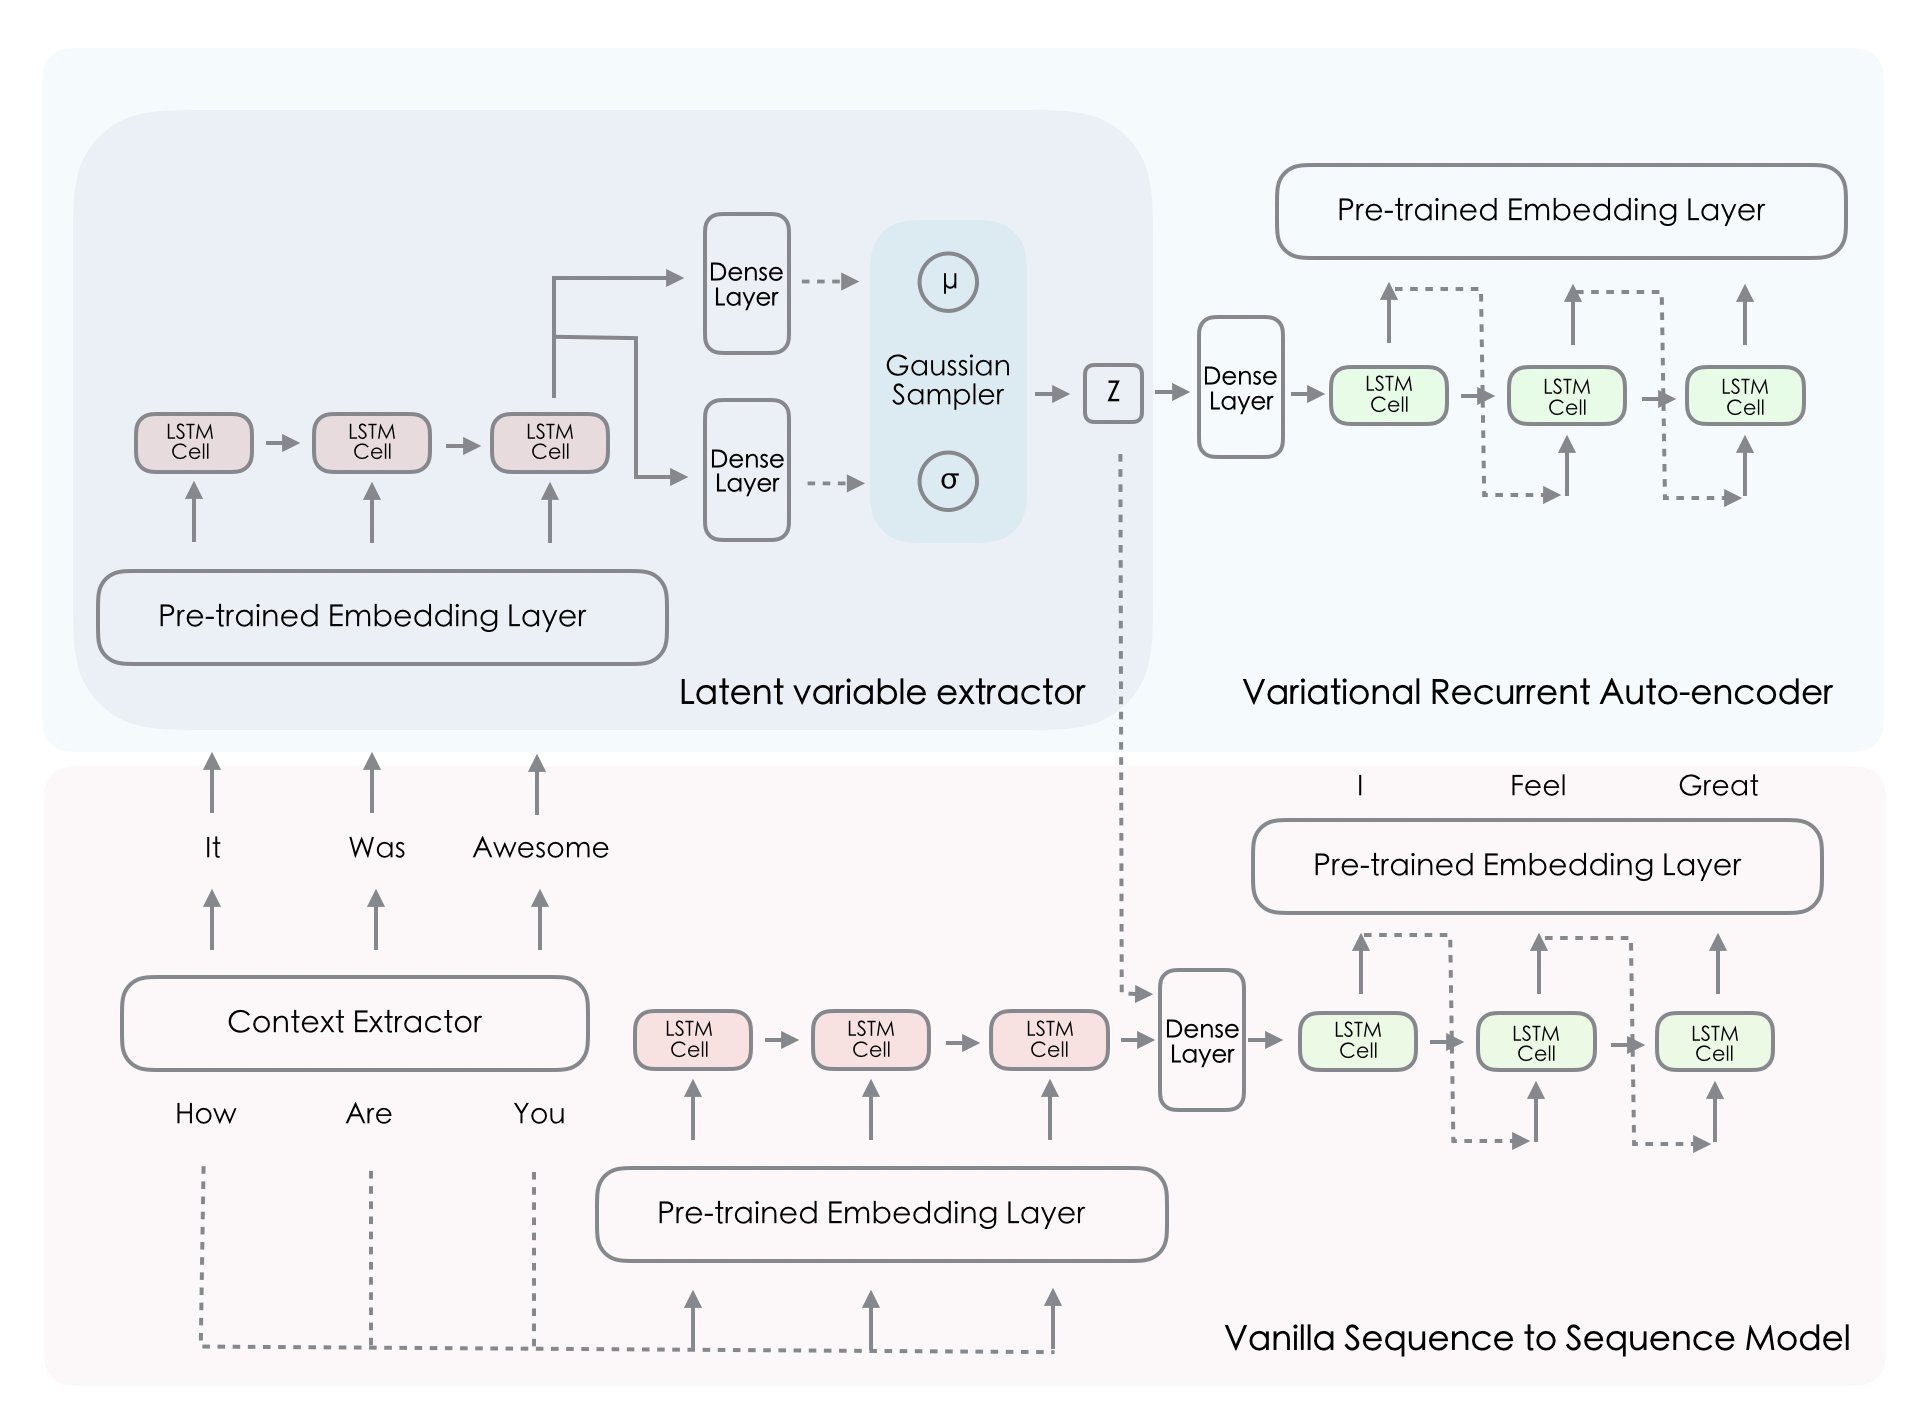
\includegraphics[width=0.8\textwidth]{proposed.png}
\caption{Proposed Method}
\label{fig:proposed}
\end{figure*}

\subsection{Incorporating latent variables in the training of Seq2Seq model}

Following the work in \cite{vnmt}, which introduces a variational model for neural machine translation that incorporates a continuous latent variable $z$ to model the underlying semantics of sentence pairs, we can also apply it to our neural conversation model that uses the same seq2seq model. 

We can also apply the method proposed by \cite{vrnn}, that explicitly models the dependencies between latent random variables across subsequent time steps.

\section{Experiments}
\subsection{Dataset Preparation}
The dataset that we used in training basic Seq2Seq model is Cornell Movie-Dialogs Corpus \cite{corpus}, which comprises of 220,579 conversational exchanges extracted from raw movie scripts on IMDB, between 10,292 pairs of movie characters from 617 movies. 

Depends on whether the context is considered or not during the training, the dataset is treated differently For different models. For training the original seq2seq model, if a response has more than one line of sentence, we only take the first one. For example:

\begin{itemize}
\item[~] \textbf{Cameron}: \textit{Gigglepuss is playing there tomorrow night.}
\item[~] \textbf{Patrick}: \textit{So what does that give me?  I'm supposed to buy her some noodles and a book and sit around listening to chicks who can't play their instruments?}
\end{itemize}

becomes

\begin{itemize}
\item[~] \textbf{Cameron}: \textit{Gigglepuss is playing there tomorrow night.}
\item[~] \textbf{Patrick}: \textit{So what does that give me?}
\end{itemize}

On the other hand, for training VNRAE model we introduce the concept of sliding window as representation of context.


In addition, in order to fit the training tensor, we also set the limit to maximum length of each input line. The sentence length limit


Each word in a sentence is tokenized and added to the vocabulary. The total vocabulary size of the Cornell Movie-Dialogs Corpus adds up to 35,147 different words, which are used to build look-up table later in the training phase.

\subsection{Training environment}
We use 300 hidden units for each LSTM, along with the learning rate $\eta=0.001$ and momentum $\gamma=0.9$ as the hyper parameters. The training takes place in Amazon AWS EC2 instance p2.xlarge, with single NVIDIA Tesla K80 GPU and CUDA accerlation. Consider the long training time (around 4 hours per epoch if we use all the data), we decide not to sacrafice any data but reduce the number of epochs for this midway report, since a trained model can always be fine-tuned with additional epochs in the future. For the current stage, we reached a model with a 10 epochs, which seems to still have some basic chatting ability (see below).

\subsection{Various Context Sizes of Conversation}


\subsection{Results and discussion}

As shown in the figure \ref{fig:loss}, we are pretty sure that the we haven't reach the minimum of our LSTM loss function at current stage. The model still have leeway for improvement in the future given enough additional epochs.

\begin{figure}[H]
\centering
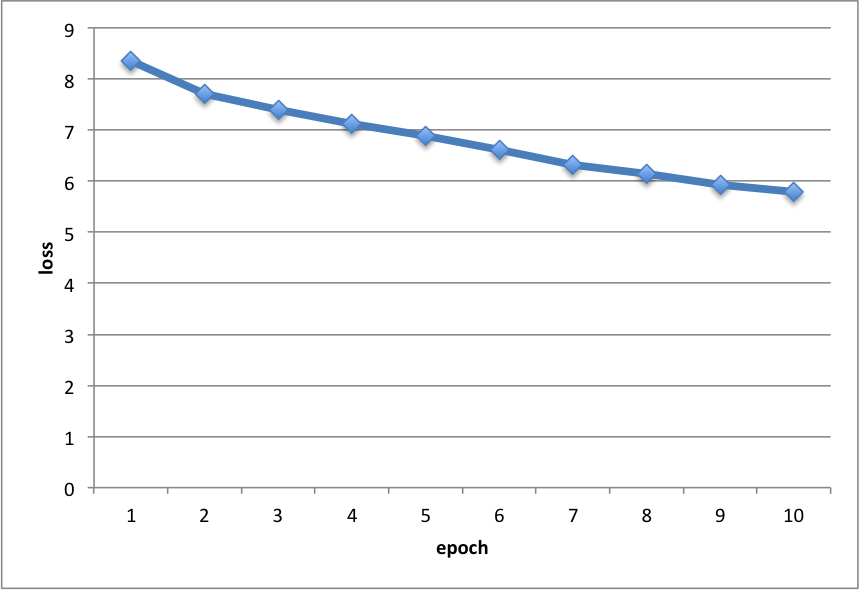
\includegraphics[width=0.4\textwidth]{loss.png}
\caption{Training of a basic Seq2Seq model}
\label{fig:loss}
\end{figure}

To demonstrate the result, here we provide a sample of conversation:

\begin{itemize}
\item[~] \textbf{Input}: \textit{Hi.}
\item[~] \textbf{Bot}: \textit{Hi.}
\item[~] \textbf{Input}: \textit{How are you?}
\item[~] \textbf{Bot}: \textit{I don't know.}
\item[~] \textbf{Input}: \textit{Why?}
\item[~] \textbf{Bot}: \textit{Because i'm a little confused.}
\item[~] \textbf{Input}: \textit{Are you a machine?}
\item[~] \textbf{Bot}: \textit{I'm not.}
\item[~] \textbf{Input}: \textit{Are you sure?}
\item[~] \textbf{Bot}: \textit{Yes.}
\item[~] \textbf{Input}: \textit{What's your name?}
\item[~] \textbf{Bot}: \textit{I'm not going to let you get away with it.}
\item[~] \textbf{Input}: \textit{You are kidding...right?}
\item[~] \textbf{Bot}: \textit{No.}
\end{itemize}

At first, the response form our vanilla Seq2Seq seems reasonable, but there are still problems. First, the model gives a weird response after we input "What's your name?" This is probably because our model doesn't reach the optimum. Second, the constrain of this model doesn't have generative ability. After few tests, we can observe that the model will always give the same response for a given input. Lastly, the Seq2Seq model only consider the short-term memory inside each sentence pairs but the long-term memory in the history of conversation. In other words, if we ask "Are you sure?", the current model will always answer "Yes" regardless the previous question. Therefore, in the future we want to see if incoporating VAE with Seq2Seq can solve these problems and improve the chatting performance.

\subsection{Incoming experiments for combining}
\subsubsection{Data and prepossessing}
For our experiments, the raw dataset including original subtitles from movies. In order to feed our data into model, we need to perform some prepossessing. We will split the sequence of communication into pair of dialogues using the information of time intervals between sentences. More specifically, if the difference of time labels for two neighborhood sentences are within several seconds, then they can form a pair of dialogue, which means the last sentence can be seen as a response to first sentence. Moreover, we will only take the first line of sentences if there are multiple lines within the last sentences. After we construct pairs of sentences, we will perform word embedding in order to turn terms in sentences into representative vectors. These vectors will be the input for our vanilla seq2seq model as well as variational recurrent auto-encoder.

\subsubsection{Training VRAE to combine with Seq2seq model}
The experiment is composed of two phases.

In the first stage, we train a VRAE with 300 hidden units on the dataset described in the last section. The dimensionality of latent spaces is to be tuned based on preliminary experiment. We will try a two dimensional latent space first for the convenience of visualization of latent units as well as saving training time. Since the optimizer is very important to the training of VRAE. We will tune the parameter of optimizer based on the lower bound of log likelihood and choose a reasonable parameter for our next experiments. If the parameter is fine tuned, we should see that the location of data points in the two-dimensional latent space distributed according some patterns instead of just randomly distributed. However, a simple two dimensional latent space may not be able to fully capture the information of dialogues. Thus, we will perform VRAE with higher dimensional multivariate Gaussian latent variables. Note that as the number of dimensions increase, we will need more training time for VRAE. Here, the capacity of model and the computing resources are a trade-off that we need to balance.

For the first stage, we will get the change of lower bound versus epochs, latent variables vector and corresponding samples draw from the latent variables for two dimensional latent space as well as a higher dimensional latent space.

In the second stage, we append the sampling vectors as context information to the dense vector of Seq2seq model. We will make a comparison between the vanilla Seq2seq model and the improved one with context information appended. Then we will test the quality of generated dialogue with quantitative BLEU score as well as qualitative human judgements.

\section{Upcoming plans}
In our proposed methods, we will incorporate context information generated by VRAE into the Seq2seq model. It is naturally to think about add more generic features of sentences more than just context information: which may include the sentiment, the semantic structure, the topic and so on.

A recent research about controllable text generation \cite{hu2017controllable} combines unstructured latent code $z$ with structured code $c$ targeting attributes of sentences to control. Here each of structured variables $c$ targets a salient and independent semantic feature of sentences. What's more, they introduced a discriminator to enforce the generator (decoder)  produce attributes coherent with the conditioned code. The learning of their model is a process of alternating the optimization of the generator and the discriminator. Their proposed model can be seen as a hybrid of vanilla VAE and wake-sleep method. Our next step involves investigating more deeply into the structured code and see if we can make improvement by incorporating GAN framework into our existing diaglog system. 

\bibliography{refs}
\bibliographystyle{icml2017}

\end{document} 


% This document was modified from the file originally made available by
% Pat Langley and Andrea Danyluk for ICML-2K. This version was
% created by Lise Getoor and Tobias Scheffer, it was slightly modified  
% from the 2010 version by Thorsten Joachims & Johannes Fuernkranz, 
% slightly modified from the 2009 version by Kiri Wagstaff and 
% Sam Roweis's 2008 version, which is slightly modified from 
% Prasad Tadepalli's 2007 version which is a lightly 
% changed version of the previous year's version by Andrew Moore, 
% which was in turn edited from those of Kristian Kersting and 
% Codrina Lauth. Alex Smola contributed to the algorithmic style files.  
